\subsection{Cache 与访存层次}

\begin{figure}[H]
  \centering
  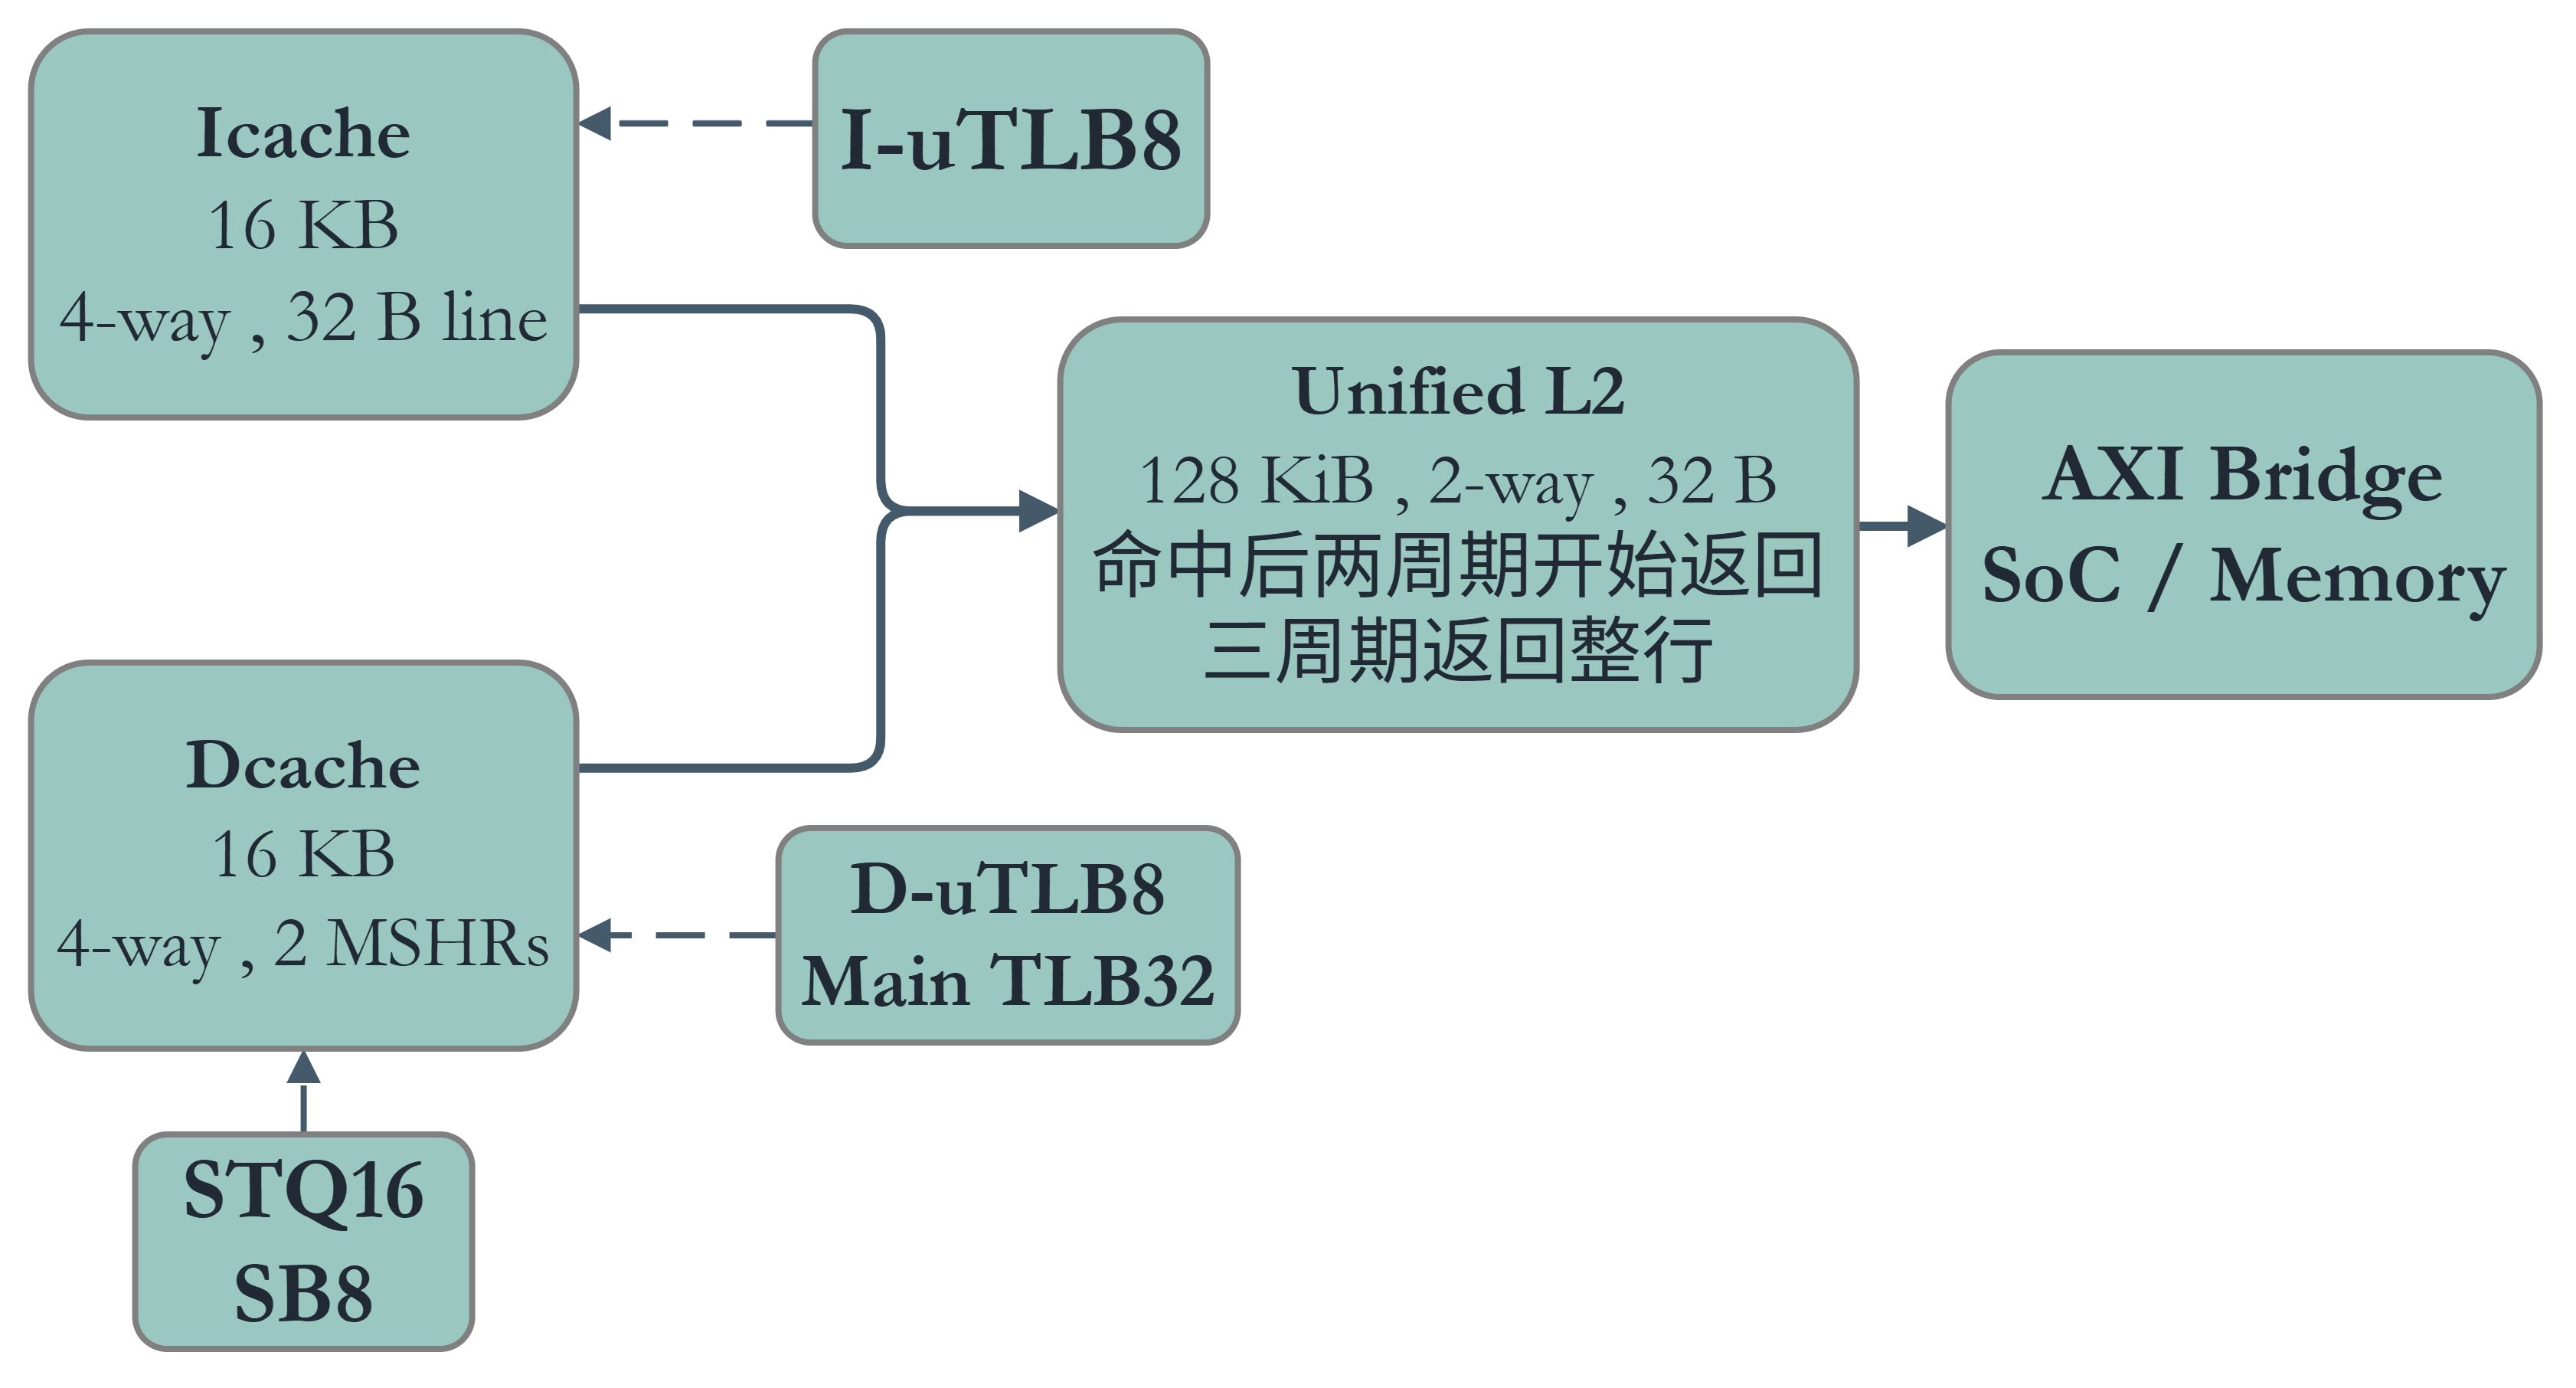
\includegraphics[width=0.95\textwidth]{figure/memory.png}
  \caption{访存架构图}
  \label{fig:memory}
\end{figure}

意味核采用 ICache/DCache、统一 L2 Cache 和 AXI 行桥的三级访问路径，并以 STQ 与 Store Buffer 分离投机 Store 和已提交 Store。

\subsubsection{一级指令缓存}

ICache 容量为 16\,KB，组织为 4 路$\times$128 组$\times$32\,B，采用 VIPT 查询。命中时向 IFU 返回完整 Cache 行；缺失时通过单一 miss 状态机向 L2 请求 refill。\texttt{cacop} 维护请求在当前事务完成后串行执行，在途返回若已因前端冲刷失效则不再写入取指流水。

\subsubsection{一级数据缓存}

DCache 同样为 16\,KiB、4 路$\times$128 组$\times$32\,B、VIPT，面向 LSU 的 Load/Store。两个 MSHR 支持 hit-under-miss，并可合并同一 Cache 行上的后续 Load。命中路径结合 STQ/SB 前递，缺失路径访问 L2；脏行替换采用写回策略。

\subsubsection{统一二级缓存}

L2 容量为 128\,KB，2 路$\times$2048 组$\times$32\,B，供 ICache 与 DCache 共享。L2 具有 I/D 独立下游读端口、4 项 victim buffer 和写回控制，可在 DCache refill 时尽早向上游返回所需数据。保守的 ICache next-line 与 DCache stream 预取在不破坏需求访问优先级的前提下减少连续访问 miss。

\subsubsection{STQ 与 Store Buffer}

\begin{itemize}
  \item \textbf{STQ（16 项）}：保存未提交 Store，按 ROB 顺序提供 Load 相关性检查与数据前递；错误路径冲刷时相应投机项被清除；
  \item \textbf{Store Buffer（8 项）}：保存已提交 Store，可合并同一 Cache 行或相邻写掩码，再写入 DCache/L2；其内容在全局冲刷后继续排空。
\end{itemize}

LSU 优先检查 STQ 与 Store Buffer 前递，再访问 DCache。已确认的数据旁路可以提前完成对应 ROB 项，从而降低访存密集程序的提交阻塞。
